\documentclass[12pt]{article}

% ── Packages ──────────────────────────────────────────────────────────────
\usepackage[margin=1in]{geometry}
\usepackage{setspace}
\doublespacing
\usepackage{graphicx}
\usepackage{amsmath, amssymb}
\usepackage{booktabs}
\usepackage{hyperref}
\usepackage{float}
\usepackage{caption}
\usepackage[numbers]{natbib}
\usepackage{url}

\graphicspath{{figures/}}

% ── Title ─────────────────────────────────────────────────────────────────
\title{Optimizing Nuclear Shelter Placement Across USA\\Using a Memetic Genetic Algorithm}
% \author{Murtaza Nipplewala, Aartika Parmar, Samyak Shah}
\author{
Murtaza Nipplewala, Aartika Parmar, Samyak Shah \\
\small \href{https://github.com/MurtazaN/nuclear_shelter_location.git}{\nolinkurl{GitHub: https://github.com/MurtazaN/nuclear_shelter_location.git}}
}
\date{}

\begin{document}
\maketitle

% ══════════════════════════════════════════════════════════════════════════
\section{Introduction}
% ══════════════════════════════════════════════════════════════════════════

The threat of nuclear conflict, while diminished since the end of the Cold War, remains a critical concern for national defense planning. A central challenge in civil defense preparedness is determining where to locate emergency shelters so that the maximum number of civilians can reach safety within a limited time, while ensuring that the shelters themselves are not placed within areas likely to be destroyed by nuclear blasts. This problem sits at the intersection of operations research, computational intelligence, and public safety policy.

From an optimization perspective, the nuclear shelter placement problem can be formulated as a variant of the \textit{Uncapacitated Facility Location Problem} (UFLP). In the classical UFLP, a decision-maker must choose a subset of candidate sites from a large set of potential locations to open facilities, with the goal of minimizing the total cost of serving all demand points while balancing facility opening costs against transportation costs \cite{cornuejols1990}. The UFLP is known to be NP-hard, meaning that exact solutions become computationally intractable as the number of candidate sites grows into the tens of thousands. This characteristic makes metaheuristic approaches, such as genetic algorithms, particularly attractive.

Genetic algorithms (GAs) are population-based search methods inspired by Darwinian natural selection. A population of candidate solutions evolves over successive generations through selection, crossover, and mutation operators, guided by a fitness function that encodes the objective \cite{holland1992}. GAs have been successfully applied to facility location problems in a variety of domains, including warehouse placement, emergency service siting, and telecommunications network design. Importantly, Jaramillo et al.\ \cite{jaramillo2002} demonstrated that genetic algorithms can effectively solve large-scale UFLP instances where exact methods are infeasible, achieving near-optimal solutions in practical computation time. Their work showed that GAs can balance the trade-off between facility opening costs and demand coverage, a balance that is directly analogous to our problem of placing the fewest shelters while maximizing population coverage.

In this project, we apply a memetic genetic algorithm---a GA enhanced with local search---to the problem of siting nuclear shelters across the continental United States. Our formulation incorporates three real-world constraints and objectives that go beyond the classical UFLP. First, shelters must be placed outside nuclear blast zones, which we model using yield-specific exclusion radii derived from the Hopkinson--Cranz cube-root scaling law \cite{glasstone1977}. Second, shelters should be located near urban infrastructure to facilitate construction and supply logistics. Third, the total number of shelters should be minimized to reflect realistic budget constraints. We encode these objectives into a weighted fitness function and compare the GA's performance against a greedy heuristic baseline.

The remainder of this paper is organized as follows. Section~2 describes our methodology, including the data sources, problem formulation, fitness function design, genetic algorithm operators, and hyperparameter tuning procedure. Section~3 presents the results of our experiments. Section~4 discusses the strengths and limitations of our approach and suggests directions for future work.


% ══════════════════════════════════════════════════════════════════════════
\section{Methods}
% ══════════════════════════════════════════════════════════════════════════

% ── 2.1 Data Sources ─────────────────────────────────────────────────────
\subsection{Data Sources}

Our approach relies on three primary datasets. The first is a U.S.\ Census population dataset organized by ZIP code, obtained from Kaggle \cite{kaggle_census}. The raw dataset contains approximately 1.6 million rows broken down by age and gender demographics. We aggregated these to the ZIP code level, yielding 32,832 unique ZIP codes with nonzero populations. Each ZIP code was geocoded to latitude and longitude coordinates using the \texttt{pgeocode} library \cite{pgeocode}.

The second dataset is a catalog of 1,087 nuclear targets across the United States, sourced from the Nuclear War Map project by Christopher Minson LLC \cite{nuclearwarmap}. Each target includes geographic coordinates, weapon yield (ranging from 10 to 2,000 kilotons), and burst type (air burst or surface burst). These attributes are essential for computing yield-specific blast exclusion zones.

The third dataset is a catalog of 3,601 U.S.\ urban areas with centroid coordinates, obtained from Kaggle \cite{kaggle_urban}. We use this dataset to compute infrastructure accessibility scores, reflecting the practical consideration that shelters built near urban centers are easier to supply, staff, and maintain.

% ── 2.2 Problem Formulation ──────────────────────────────────────────────
\subsection{Problem Formulation}

We model the nuclear shelter placement problem as a constrained variant of the Uncapacitated Facility Location Problem. Let $\mathcal{Z} = \{z_1, z_2, \ldots, z_N\}$ denote the set of candidate ZIP codes, where $N$ is the number of safe candidates after blast zone exclusion. Each candidate $z_i$ has an associated population $p_i$ and geographic coordinates $(\text{lat}_i, \text{lon}_i)$. A solution is a binary vector $\mathbf{x} \in \{0, 1\}^N$, where $x_i = 1$ indicates that a shelter is placed at ZIP code $z_i$.

\subsubsection{Blast Zone Exclusion}

Before optimization begins, we exclude all ZIP codes that fall within the blast radius of any nuclear target. Rather than applying a uniform exclusion radius, we compute target-specific radii using the Hopkinson--Cranz cube-root scaling law from Glasstone and Dolan \cite{glasstone1977}:
\begin{equation}
R(Y) = R_{\text{ref}} \cdot Y^{1/3} \cdot \beta
\end{equation}
where $R_{\text{ref}}$ is the reference radius at 1 kiloton for a given overpressure threshold, $Y$ is the weapon yield in kilotons, and $\beta$ is a burst-type multiplier ($\beta = 1.0$ for surface bursts, $\beta = 1.25$ for air bursts). We use the 5 psi overpressure threshold ($R_{\text{ref}} = 0.292$ miles), corresponding to severe structural damage and residential collapse. This filtering reduces the candidate set from 32,832 to 30,962 ZIP codes, excluding 1,870 that fall within blast zones.

\subsubsection{Coverage Model}

A ZIP code $z_i$ is considered ``covered'' if at least one selected shelter is within a 50-mile service radius, computed using the Haversine distance formula. We precompute a sparse boolean coverage matrix $\mathbf{C} \in \{0, 1\}^{N \times N}$, where $C_{ij} = 1$ if $z_i$ is within 50 miles of $z_j$. This matrix contains approximately 4.8 million nonzero entries (0.50\% density) and enables efficient coverage evaluation through sparse matrix--vector products.

\subsubsection{Fitness Function}

The fitness of a solution $\mathbf{x}$ is a weighted combination of three normalized objectives:
\begin{equation}
f(\mathbf{x}) = w_{\text{cov}} \cdot \frac{\sum_{i \in \text{covered}} p_i}{\sum_{i=1}^{N} p_i} + w_{\text{infra}} \cdot \overline{s}_{\text{infra}}(\mathbf{x}) - w_{\text{cost}} \cdot \frac{|\mathbf{x}|}{N}
\label{eq:fitness}
\end{equation}
where the first term is the population coverage ratio, the second is the mean infrastructure accessibility score of selected shelters, and the third is a cost penalty proportional to the number of shelters. The infrastructure score for each candidate is computed as $s_i = \max_{u \in \mathcal{U}} \exp(-d(z_i, u) / 50)$, where $\mathcal{U}$ is the set of urban areas and $d(\cdot, \cdot)$ is the Haversine distance in miles. We set $w_{\text{cov}} = 0.7$, $w_{\text{infra}} = 0.2$, and $w_{\text{cost}} = 0.1$, reflecting the primary importance of population coverage.

% ── 2.3 Genetic Algorithm ────────────────────────────────────────────────
\subsection{Genetic Algorithm}

Our primary optimization method is a memetic genetic algorithm with several enhancements over a standard GA.

\subsubsection{Chromosome Encoding and Fixed-K Constraint}

Each chromosome is a binary vector of length $N = 30{,}962$, where a 1 at position $i$ indicates a shelter at ZIP code $z_i$. To enforce a budget constraint, we use a \textit{fixed-K} encoding: every chromosome maintains exactly $K$ shelters throughout the evolutionary process, where $K$ is derived from a target shelter ratio parameter. This eliminates the need for penalty-based budget enforcement and ensures that all solutions in the population are budget-feasible.

\subsubsection{Population Initialization and Greedy Seeding}

The initial population is constructed in two phases. First, 25\% of the population is seeded with the greedy heuristic solution and perturbed variants of it (created by randomly swapping a small number of selected and unselected shelters). The remaining 75\% of individuals are initialized by randomly selecting $K$ positions. This seeding strategy gives the GA a strong starting point while maintaining population diversity.

\subsubsection{Selection}

We use tournament selection with a configurable tournament size. In each tournament, a small subset of the population is sampled uniformly at random, and the individual with the highest fitness is selected as a parent. This method provides adjustable selection pressure without requiring the population to be sorted.

\subsubsection{Crossover}

We employ uniform crossover, where each gene is independently inherited from one parent or the other with equal probability. Because uniform crossover can disrupt the fixed-K constraint, we apply a repair operator after each crossover: if the offspring has too many shelters, randomly selected excess shelters are removed; if too few, randomly selected empty positions are activated.

\subsubsection{Mutation}

Rather than independent bit flips, which would violate the fixed-K constraint, we use \textit{swap mutation}. The number of swaps is drawn from a binomial distribution $\text{Bin}(K, p_m)$, where $p_m$ is the mutation rate. Each swap simultaneously deactivates one selected shelter and activates one unselected position, preserving the total count.

\subsubsection{Elitism}

The top $e$ individuals (by fitness) from each generation are copied unchanged into the next generation, ensuring that the best-known solution is never lost. In our experiments, $e$ ranges from 1 to 3.

\subsubsection{Local Search (Memetic Component)}

After fitness evaluation in each generation, the top 3 elite individuals undergo a randomized 1-swap hill-climbing procedure. For each elite, 12 random single-swap neighbors are evaluated, and the elite is replaced by the best-improving neighbor (if any improvement is found). This memetic step refines promising solutions without the computational cost of applying local search to the entire population.

\subsubsection{Adaptive Mutation Rate}

When enabled, the mutation rate decays linearly from the base rate to one-fifth of the base rate over the course of evolution, encouraging broad exploration early and fine-tuning later. Additionally, if the best fitness has not improved for 15 consecutive generations (a stagnation event), the mutation rate is temporarily boosted to three times the base rate to escape local optima.

% ── 2.4 Greedy Baseline ─────────────────────────────────────────────────
\subsection{Greedy Heuristic Baseline}

As a baseline for comparison, we implement a greedy set-cover heuristic. At each iteration, the algorithm selects the candidate ZIP code that covers the most currently uncovered population (measured as the marginal gain in covered population). Infrastructure scores serve as a tiebreaker, adding a small bonus of $10 \times s_i$ to the marginal gain of candidate $i$. The algorithm runs until the shelter budget is exhausted or no further population gain is possible. This greedy approach is computationally efficient, running in time proportional to $K$ iterations of sparse matrix--vector products, but it is inherently myopic and cannot escape locally optimal selections.

% ── 2.5 Hyperparameter Tuning ────────────────────────────────────────────
\subsection{Hyperparameter Tuning with Optuna}

To identify effective hyperparameter configurations for the GA, we use Optuna \cite{optuna2019}, a Bayesian hyperparameter optimization framework. Optuna uses a Tree-structured Parzen Estimator (TPE) to guide the search through the hyperparameter space, efficiently balancing exploration and exploitation across trials.

We tune seven hyperparameters: population size (60--160), number of generations (80--260), mutation rate (0.005--0.05, log scale), crossover rate (0.70--0.95), tournament size (2--4), target shelter ratio (0.003--0.02, log scale), and elitism count (1--3). Each trial evaluates the sampled configuration across three random seeds, and the mean fitness across seeds is used as the objective to favor robust parameter settings. The study is persisted in a SQLite database, enabling incremental refinement across multiple tuning sessions.

% ── 2.6 Software and Implementation ─────────────────────────────────────
\subsection{Software and Implementation}

The system is implemented in Python and relies on NumPy \cite{numpy2020} for vectorized numerical operations, SciPy \cite{scipy2020} for sparse matrix representations, Pandas \cite{pandas2020} for data manipulation, and Matplotlib \cite{matplotlib2007} for visualization. The \texttt{pgeocode} library \cite{pgeocode} is used for ZIP code geocoding, and Optuna \cite{optuna2019} is used for hyperparameter optimization. All distance calculations use the Haversine formula for great-circle distance on a spherical Earth. The coverage matrix is stored in compressed sparse row (CSR) format and computed in chunks of 2,000 ZIP codes to avoid memory overflow. All experiments were run with a fixed random seed of 42 for reproducibility.


% ══════════════════════════════════════════════════════════════════════════
\section{Results}
% ══════════════════════════════════════════════════════════════════════════

% ── 3.1 Optuna Tuning ────────────────────────────────────────────────────
\subsection{Hyperparameter Tuning Results}

We ran five Optuna trials, each evaluating a sampled hyperparameter configuration across three random seeds. Table~\ref{tab:optuna} summarizes the results of all trials, sorted by mean fitness.

\begin{table}[H]
\centering
\caption{Optuna hyperparameter tuning results across five trials.}
\label{tab:optuna}
\begin{tabular}{ccccccc}
\toprule
Trial & Fitness & Coverage (\%) & Pop.\ Size & Generations & Mut.\ Rate & Tourn.\ Size \\
\midrule
4 & \textbf{0.8522} & 99.77 & 40 & 220 & 0.0052 & 5 \\
2 & 0.8514 & 99.65 & 110 & 120 & 0.0056 & 3 \\
1 & 0.8507 & 99.63 & 120 & 260 & 0.0166 & 7 \\
0 & 0.8501 & 99.36 & 50 & 200 & 0.0245 & 5 \\
3 & 0.8492 & 99.75 & 80 & 260 & 0.0296 & 2 \\
\bottomrule
\end{tabular}
\end{table}

The best trial (Trial 4) achieved a mean fitness of 0.8522 with a population size of 40, 220 generations, a low mutation rate of 0.0052, crossover rate of 0.748, tournament size of 5, and an elitism count of 3. Notably, the best-performing configuration used a relatively small population size but ran for more generations, suggesting that sustained refinement is more valuable than broad initial exploration for this problem. Lower mutation rates consistently outperformed higher ones, indicating that the search landscape rewards incremental improvement over disruptive exploration.

% ── 3.2 Final GA vs Greedy ────────────────────────────────────────────────
\subsection{GA vs.\ Greedy Baseline Comparison}

Using the best hyperparameters from Optuna, we ran the final GA with a fixed budget of $K = 319$ shelters (corresponding to a target shelter ratio of approximately 1.03\% of candidate ZIP codes). Table~\ref{tab:comparison} compares the GA and greedy baseline on all evaluation metrics.

\begin{table}[H]
\centering
\caption{Final comparison of the memetic GA and greedy heuristic baseline, both constrained to 319 shelters.}
\label{tab:comparison}
\begin{tabular}{lcc}
\toprule
Metric & GA (Optuna-tuned) & Greedy Baseline \\
\midrule
Shelters placed       & 319              & 319              \\
Population covered    & 258,737,147      & 260,055,826      \\
Coverage (\%)         & 97.58            & 98.08            \\
Infrastructure score  & 0.856            & 0.817            \\
Cost ratio            & 0.0103           & 0.0103           \\
\textbf{Fitness}      & \textbf{0.8532}  & 0.8489           \\
Runtime (seconds)     & 88.0             & 3.1              \\
\bottomrule
\end{tabular}
\end{table}

The GA outperformed the greedy baseline on the composite fitness metric by 0.51\%, achieving a fitness of 0.8532 compared to 0.8489. This improvement is driven primarily by the GA's superior infrastructure accessibility score (0.856 vs.\ 0.817), indicating that the evolutionary search found shelter configurations that are better positioned relative to urban centers. The greedy heuristic, by contrast, achieved slightly higher raw population coverage (98.08\% vs.\ 97.58\%), which is expected because greedy selection directly maximizes marginal population gain at each step without considering infrastructure proximity.

Figure~\ref{fig:comparison} presents a side-by-side bar chart of the key metrics. The trade-off between coverage and infrastructure quality is evident: the greedy approach covers approximately 1.3 million more people but places shelters in less accessible locations.

\begin{figure}[H]
\centering
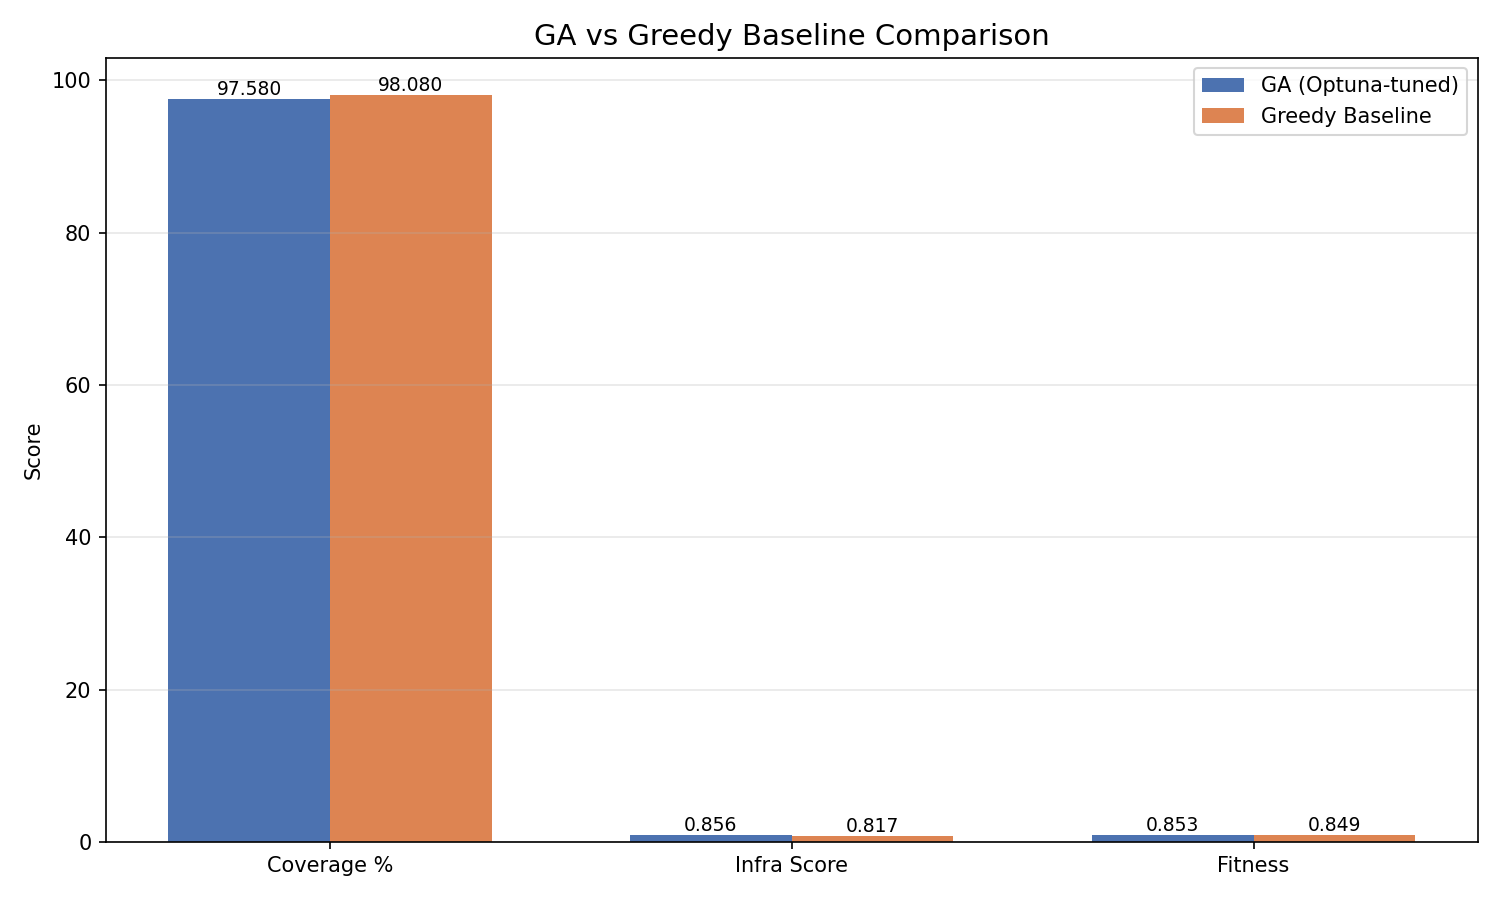
\includegraphics[width=0.85\textwidth]{comparison_plot.png}
\caption{Comparison of GA and greedy baseline on coverage percentage, infrastructure score, and composite fitness.}
\label{fig:comparison}
\end{figure}

% ── 3.3 Convergence Behavior ─────────────────────────────────────────────
\subsection{Convergence Behavior}

Figure~\ref{fig:convergence} shows the convergence curves for the final GA run over 220 generations. The best fitness curve exhibits rapid initial improvement during the first 30 generations, rising from 0.8490 (the greedy seed fitness) to approximately 0.8501. Improvement continues at a slower rate through the remaining generations, with the final best fitness of 0.8532 reached at generation 217. The average population fitness follows a similar trend, rising from 0.724 at generation 0 to approximately 0.850 by generation 30, and then gradually converging toward the best fitness through the remainder of the run.

The initial jump in average fitness (from 0.724 to 0.814 between generations 0 and 1) reflects the strong influence of greedy seeding: the seeded individuals and their perturbed variants quickly dominate the population through selection. The slow but consistent improvement after generation 30 demonstrates the value of the memetic local search component, which continues to refine elite solutions even after the global search operators have largely converged.

\begin{figure}[H]
\centering
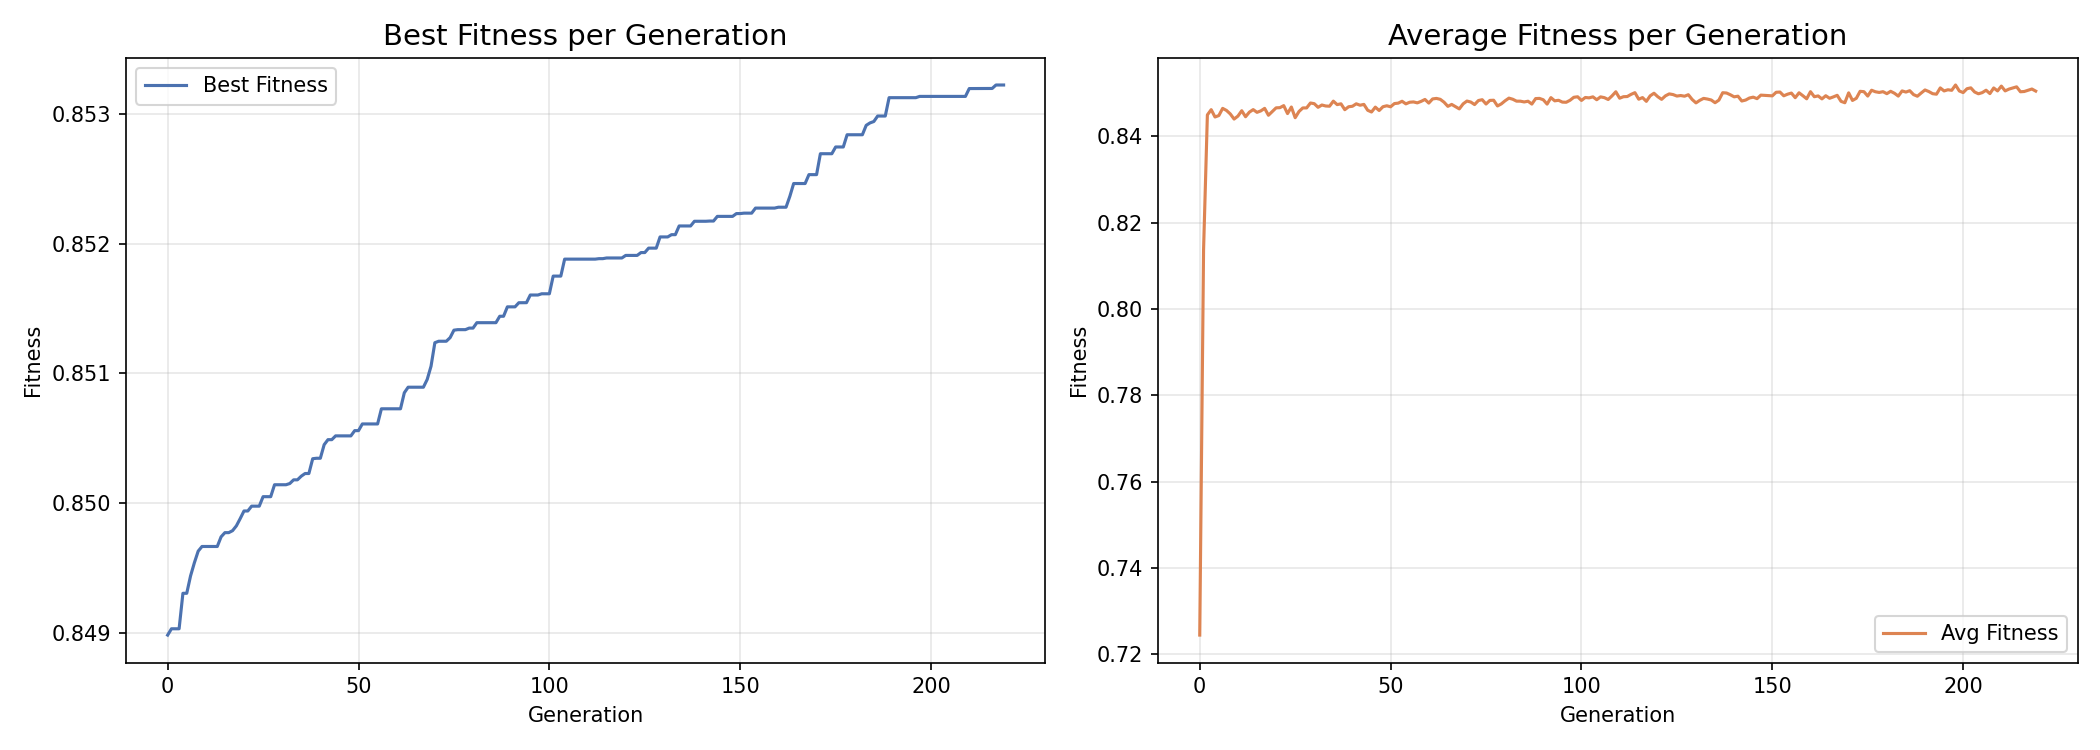
\includegraphics[width=\textwidth]{convergence_plot.png}
\caption{Convergence of the GA over 220 generations. Left: best fitness per generation. Right: average population fitness per generation.}
\label{fig:convergence}
\end{figure}

% ── 3.4 Shelter Map ──────────────────────────────────────────────────────
\subsection{Geographic Distribution of Shelters}

Figure~\ref{fig:map} shows the geographic distribution of the 319 shelters selected by the GA, overlaid on all 30,962 candidate ZIP codes. The shelters are concentrated in and around major population centers, as expected from the coverage-dominated fitness function. Dense clusters appear in the Northeast corridor, the Great Lakes region, California, Texas, and Florida. Rural areas of the Mountain West and Great Plains are served by more sparsely distributed shelters that each cover large geographic areas due to the 50-mile service radius.

\begin{figure}[H]
\centering
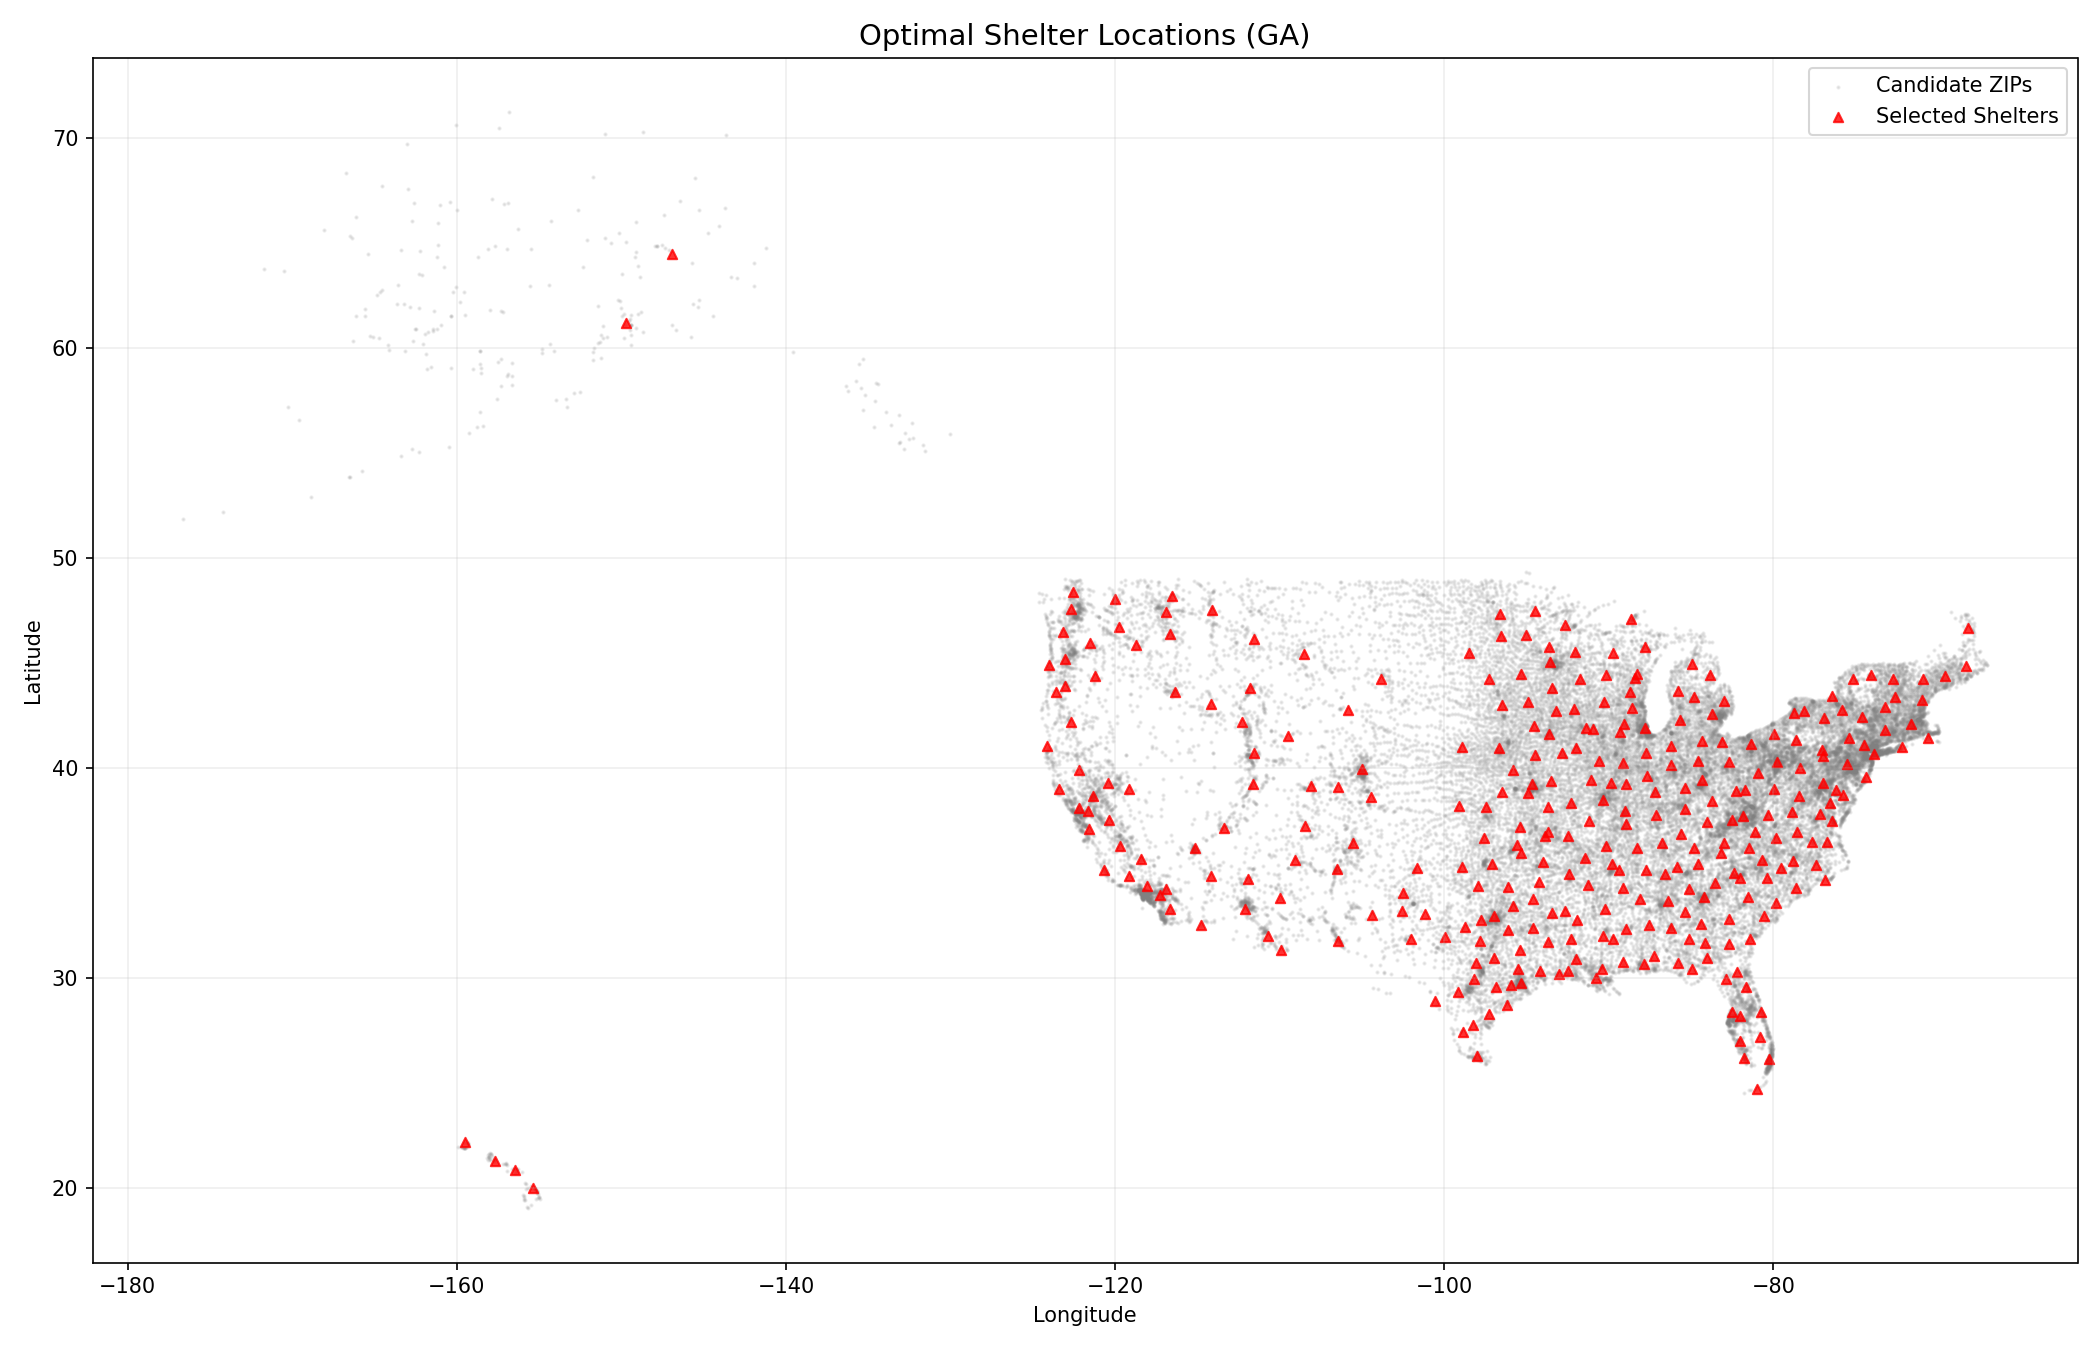
\includegraphics[width=0.9\textwidth]{shelter_map.png}
\caption{Geographic distribution of 319 shelters (red triangles) selected by the GA, with all candidate ZIP codes shown in gray.}
\label{fig:map}
\end{figure}


% ══════════════════════════════════════════════════════════════════════════
\section{Conclusions}
% ══════════════════════════════════════════════════════════════════════════

In this project, we developed a memetic genetic algorithm for the nuclear shelter location problem, formulated as a constrained variant of the Uncapacitated Facility Location Problem. Our approach integrates yield-specific blast zone exclusion, population coverage maximization, infrastructure accessibility scoring, and budget-constrained optimization into a single evolutionary framework.

The GA achieved a composite fitness of 0.8532, outperforming the greedy heuristic baseline (0.8489) by 0.51\%. While the margin is modest, the improvement is significant in that it reflects a fundamentally different trade-off: the GA sacrifices a small amount of raw population coverage (97.58\% vs.\ 98.08\%) in exchange for substantially better infrastructure accessibility (0.856 vs.\ 0.817). In a real-world civil defense scenario, this trade-off could be meaningful, as shelters in more accessible locations are easier to supply, evacuate from, and maintain.

Several design decisions contributed to the GA's effectiveness. The fixed-K chromosome encoding eliminated budget infeasibility, allowing all genetic operators to produce valid solutions without penalty-based enforcement. Greedy seeding provided a strong initial population that accelerated convergence, while the memetic local search component enabled continued refinement after the population-level search had largely converged. The use of Optuna for hyperparameter tuning identified a configuration that favored low mutation rates and moderate selection pressure, aligning with the relatively smooth fitness landscape of this problem.

Our approach also has limitations. The fitness function uses a simple weighted sum of three objectives, and the relative weights ($w_{\text{cov}} = 0.7$, $w_{\text{infra}} = 0.2$, $w_{\text{cost}} = 0.1$) were set by domain intuition rather than systematic multi-objective optimization. A Pareto-based approach (e.g., NSGA-II) could reveal the full set of trade-offs between coverage, infrastructure quality, and cost. Additionally, our coverage model treats all populations within 50 miles as equally served, without modeling road networks, travel time, or shelter capacity. The GA's runtime of 88 seconds, while practical, is approximately 28 times slower than the greedy baseline; for larger problem instances, more efficient evaluation strategies (such as batch GPU computation or surrogate-assisted fitness approximation) may be necessary.

Future work could extend this approach in several directions. Incorporating road network travel time instead of Haversine distance would produce more realistic coverage estimates. Capacity constraints at each shelter would transform the problem into a capacitated facility location variant, which is more realistic but also more computationally demanding. Multi-objective optimization using Pareto fronts would allow decision-makers to visualize the full range of coverage-cost-accessibility trade-offs rather than committing to a single weighting scheme. Finally, the adaptive mutation mechanism could be replaced with more sophisticated diversity maintenance techniques, such as fitness sharing or island-model parallelism, to further reduce premature convergence.

Despite these limitations, our results demonstrate that a well-designed memetic genetic algorithm can effectively solve large-scale facility location problems with real-world constraints, producing solutions that balance multiple competing objectives more effectively than a simple greedy heuristic.


% ══════════════════════════════════════════════════════════════════════════
% Works Cited
% ══════════════════════════════════════════════════════════════════════════

\begin{thebibliography}{99}

\bibitem{cornuejols1990}
G.~Cornu\'{e}jols, G.~Nemhauser, and L.~Wolsey,
``The uncapacitated facility location problem,''
in \textit{Discrete Location Theory}, P.~Mirchandani and R.~Francis, Eds.
New York: Wiley, 1990, pp.~119--171.

\bibitem{holland1992}
J.~H.~Holland,
\textit{Adaptation in Natural and Artificial Systems},
2nd ed. Cambridge, MA: MIT Press, 1992.

\bibitem{jaramillo2002}
J.~H.~Jaramillo, J.~Bhadury, and R.~Batta,
``On the use of genetic algorithms to solve location problems,''
\textit{Computers \& Operations Research}, vol.~29, no.~6, pp.~761--779, 2002.

\bibitem{glasstone1977}
S.~Glasstone and P.~J.~Dolan,
\textit{The Effects of Nuclear Weapons}, 3rd ed.
Washington, DC: U.S. Department of Defense and U.S. Department of Energy, 1977.

\bibitem{optuna2019}
T.~Akiba, S.~Sano, T.~Yanase, T.~Ohta, and M.~Koyama,
``Optuna: A next-generation hyperparameter optimization framework,''
in \textit{Proceedings of the 25th ACM SIGKDD International Conference on Knowledge Discovery \& Data Mining}, 2019, pp.~2623--2631.

\bibitem{kaggle_census}
``US Population by Zip Code,''
Kaggle. [Online]. Available: \url{https://www.kaggle.com/datasets/census/us-population-by-zip-code}

\bibitem{nuclearwarmap}
C.~Minson,
``Nuclear War Map,'' Christopher Minson LLC. [Online]. Available: \url{https://nuclearwarmap.com}

\bibitem{kaggle_urban}
``United States Urban Areas Dataset,''
Kaggle. [Online]. Available: \url{https://www.kaggle.com/datasets/opendata500/united-states-urban-areas}

\bibitem{numpy2020}
C.~R.~Harris \textit{et al.},
``Array programming with NumPy,''
\textit{Nature}, vol.~585, pp.~357--362, 2020.

\bibitem{scipy2020}
P.~Virtanen \textit{et al.},
``SciPy 1.0: Fundamental algorithms for scientific computing in Python,''
\textit{Nature Methods}, vol.~17, pp.~261--272, 2020.

\bibitem{pandas2020}
W.~McKinney,
``Data structures for statistical computing in Python,''
in \textit{Proceedings of the 9th Python in Science Conference}, 2010, pp.~56--61.

\bibitem{matplotlib2007}
J.~D.~Hunter,
``Matplotlib: A 2D graphics environment,''
\textit{Computing in Science \& Engineering}, vol.~9, no.~3, pp.~90--95, 2007.

\bibitem{pgeocode}
``pgeocode: Postal code geocoding and distance calculations,''
[Online]. Available: \url{https://github.com/symerio/pgeocode}

\end{thebibliography}

\end{document}
